\chapter{基于属性信息聚合的广域网络路由异常检测研究}

在先前章节的实验中,传统的图卷积网络在广域网数据集中展现出计算复杂度过高的问题,并存在对未知节点的泛化能力的不足的缺陷。本章节将从基于信息聚合的图网络算法入手,以 GraphSAGE 为基本框架,将数据集包含的路由特征的拓展到该模型中。

% 15 页
% 魔改 GraphSAGE
% https://toutiao.io/posts/ydj46sp/preview

\section{研究背景}

% 1.5 页

近年来,随着卷积神经网络的发展,一些研究注意到了卷积在传统的基于图像的领域具有提取局部特征的良好特性,而基于图卷积模型的出现更是将卷积的思想带入了图网络领域:利用结合相邻节点的信息和自身信息的方式,能够得到图网络自身的局部表示\citing{scarselli2008graph}。基于以上思想,将图卷积运用在广域网络的路由数据中一种可行的方案。

然而,图卷积网络自身的运算量非常巨大,在具有大量节点的数据集上对于一个多层的图卷积网络的临接矩阵做卷积操作,在实际场景中很有可能超出可行的运算能力。此外,图模型中基于 GNN 的架构,例如 Deep Walk 和 GCN 等模型,通常需要在数据发生更新的时候对整个图进行重新学习,由于本研究涉及到的路由数据集所包含的图结构过于庞大,而异常检测的任务决定了模型需要一段时间后进行重新训练,这将严重阻碍模型在实际生产环境中的工作效率\citing{hamilton2017inductive}。

因而一种称为 GraphSAGE 的基于邻接节点采样的方法\citing{hamilton2017inductive}被提出。它通过预先对节点的邻居进行采样,从而降低了后续特征聚合获得嵌入需要处理的节点数量,另外,该模型的参数量是受参数控制且恒定的,不会随着图网络规模的增加而不断扩张,这使得该模型在应对路由条目不断增长的互联网路由表上具有一定优势。

然而,GraphSAGE 模型的邻居聚合一般使用基于均值的函数,没有考虑到不同的邻居节点应当对特征具有不同的贡献,该模型在采样阶段和损失的计算上也存在类似的问题,一项研究指出,对于具有一定路径拓扑的路由网络的场景而言,使用这样的计算方式并不合适\citing{el2022deep}。因此,如何设计聚合模型以针对性地学习与路径相关的特征,是一个值得探讨的研究话题。

为此,本章从经典的 GraphSAGE 模型出发,根据实际场景对该模型的采样方法、聚合函数、损失函数等关键模块进行了分析,并据此提出了对应的基于路由生成的图结构的路径特征的表示方法,这种方法利用路径信息对算法中的各组成部分赋予不同的权重,相比于典型的 GraphSAGE 模型能够反映出路径所导致的邻居节点间的不同,从而达到提升异常检测模型准确性的目的。

综上所述,本章节提出的模型贡献如下:

\begin{enumerate}
    \item 将属性信息聚合的图网络算法应用在网络路由的图数据集上,降低了图网络算法的计算开销,并使得模型在生产环境中的高效更新成为了可能。
    \item 设计了一种针对网络路由的图结构的邻居特征聚合算法和对应的损失函数,能够有效地利用数据集中的路径特征。
    \item 设计了一种根据路径信息采样邻居特征的邻居采样算法,从而更有效地从原始图网络中采样获得更具代表性的子图。
\end{enumerate}


\section{模型设计及实现}

\subsection{模型结构}

\begin{figure}[h]
    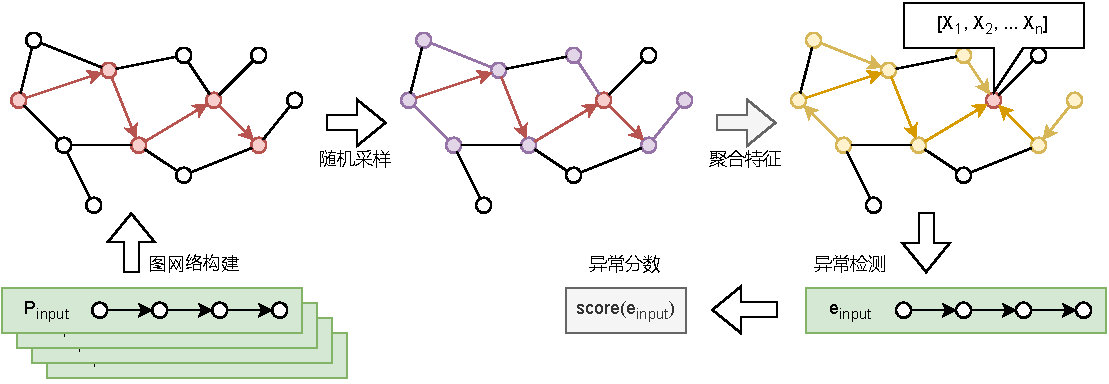
\includegraphics[width=\linewidth]{chapter/c4_images/c4_model.pdf}
    \caption{模型结构图}
    \label{c4_model}
\end{figure}

这一节的模型架构将以 GraphSAGE 模型为基础,通过对它的三个重要部分进行探讨,并针对广域网络的路由数据的特点,本研究从路径的角度出发分别提出对应的利用数据集中路径信息的方法。

如图 \ref{c4_model} 所示,本章提出的模型的结构包括了随机采样、聚合特征、异常检测三个部分,它的输入是一套网络路由数据集,首先输出对应数据集在图上的嵌入,最后通过异常检测输出对路由系统中路径更新的异常分数。

\begin{enumerate}
    \item 随机采样:该部分通过已知的路径信息优化随机采样的概率,从而实现有权重且权重基于路径信息的随机采样。
    \item 聚合特征:该部分通过引入路径带来的差异,对邻居间信息的聚合方式进行了调整,实现了基于路径权重的邻居聚合。
    \item 异常检测:该部分通过前序模型获得的嵌入,对比新路径的嵌入从而进行异常检测。
\end{enumerate}

\subsection{模型分析}

本文选取 GraphSAGE 作为模型的框架,是由于它具有以下特性:

\begin{enumerate}
    \item 训练数据通过采样获得。传统的图神经网络在面对网络路由等大规模的数据集上普遍存在性能不足的问题,GraphSAGE 通过采样子图的方式减小了需要计算的图网络矩阵尺寸,从而减少了性能开销。
    \item 聚合和采样函数具备调整空间。GraphSAGE 模型在框架上仅规定了前向传播的方法,具体的聚合和采样函数是模块化的,能够在节点层面上进行调整,这使得将路径因素引入到模型中是可行的。
\end{enumerate}

然而,GraphSAGE 模型非常依赖采样函数、聚合函数、损失函数的选取,在传统的 GraphSAGE 模型中路径是不存在的,这些函数仅会引入了节点连边的拓扑差异,在上述函数中直接采用现有方法不能利用数据集中的路径特征。因此,为了能够在路由数据集上针对性地提取特征,模型应当在这三个重要部分中体现出相应的权重差异,本研究通过在算法中引入路径因素,分别为三个部分设计了对应的改进方法。

\subsection{基于节点权重的随机采样}

大部分图网络中,图中的每个节点的度值是不一致的,为了提高模型性能,GraphSAGE 模型对于一般的图网络的通用做法\citing{hamilton2017inductive} 是为每个节点采样固定数量的邻居。而基于广域网络路由架构的性质而言,即使是在分布式网络中,广域网路由系统中的自治系统会在网络中对路由有着不同程度的控制力,即它们应当从/向不同尺度的节点获取/传递特征。

在图网络中,对节点在图网络中的控制力强度的度量方法通常是中心度,而对于在路由系统的嵌入任务而言,其中的介数中心度相比之下更具有统计意义,该方法能够将节点在最短路径中出现的频次,即介数中心度作为采样指标,从而在一定程度上反映自治系统对临接节点路由的控制能力,而这种控制能力的度量在实际场景中即对应其路由异常传播的规模。

为了验证这一结论,本研究针对节点的介数中心度的分布状况进行了实验分析。实验对来自 2022 年 10,11,12 三个月份的 RIPE RIS 数据样本按照第三章所述的基于拓扑的构图方式进行了图网络生成,以便排除对等路由的影响,随后对每一个自治系统计算了其对应的介数中心度,详细的统计结果如图 \ref{c4_node-centrality} 所示,为方便展示,横坐标轴已修改为通过对数的方式呈现。

\begin{figure}[h]
    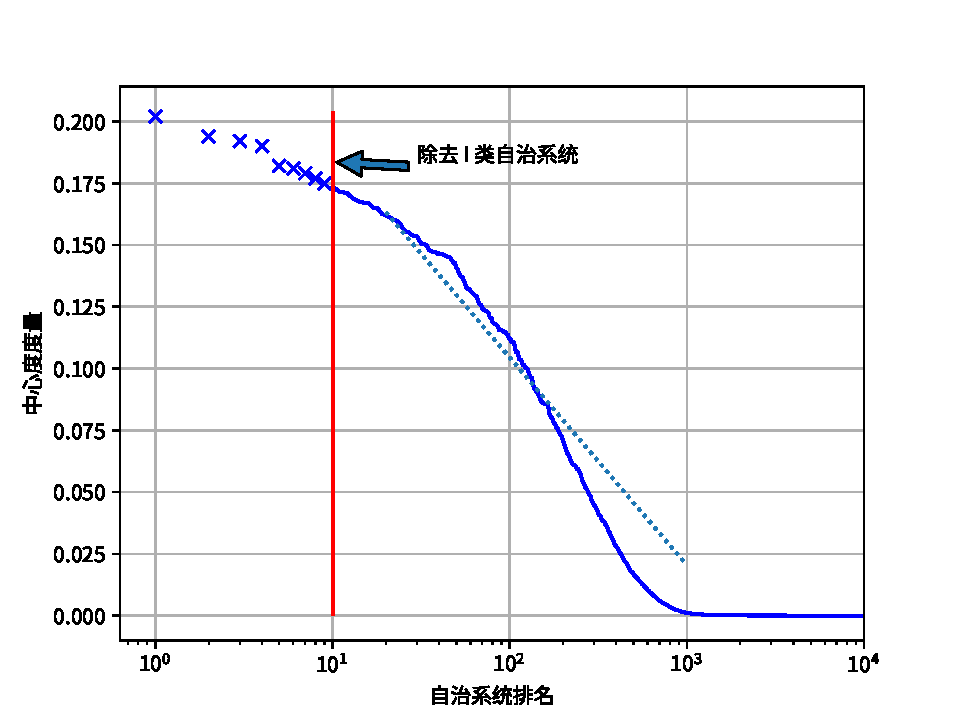
\includegraphics[width=0.8\linewidth]{chapter/c4_images/c4_node-centrality.pdf}
    \caption{RIPE 数据集中的介数中心度的分布状况}
    \label{c4_node-centrality}
\end{figure}

图 \ref{c4_node-centrality} 的结果可以反映出自治系统在中心度上的分布情况,由于 I 类自治系统自身根据定义具有很高的中心度,在去除了互联网所有 I 类自治系统(图中的红线部分右侧)后的图表趋势大致上在对数范围呈现线性下降的趋势(图中的蓝色虚线部分)。因而可以认为基于介数中心度的指标对节点进行采样和后续的特征聚合是可靠的。

因此,本章提出了如公式\ref{s3_sample_model}所示的采样模型:
\begin{equation} \label{s3_sample_model}
P_b(a) = \Sigma_{b, (a,b) \in E} \frac{\omega(a,b)}{\Sigma_{a} \omega(a,b)}, \omega(a,b) = 1 + \theta_{sample} \cdot \frac{N_{paths}^a(b)}{N_{paths}^a}
\end{equation}

其中 $\theta_{sample}$ 是一种权重值,通过它能够调整采样邻居数与其中心度的关联,当此值为 0 时,该模型退化至普通的固定采样模型。$N_{paths}^a(b)$ 是全部经由 a 节点的路径中同时经由 b 的路径数量,模型通过该式使得具有更多路径关联的邻居具有更大的采样概率。通过在原图网络上的 k 次迭代采样能够获得一个用于 k 层邻居聚合模型的子图。同时,为了限定采样规模,该采样过程由一个参数 $N_{sample}$ 控制,并决定对于一个节点而言的采样邻居数量。

根据此模型,在对邻居进行采样时将考虑到与邻居的共同路径比例,即更容易采样到具有更多公共路径的邻居信息。

\subsection{基于路由特征的邻居聚合}

一般而言,在 GraphSAGE 模型中一般使用均值聚合器方案\citing{hamilton2017inductive},即对相邻节点和本节点的上一层输出取均值,并据此进行线性变换,进而产生当前层的输出。具体的实现方式见公式\ref{graphsage_default_aggr}。
\begin{equation} \label{graphsage_default_aggr}
h^k_v \leftarrow \sigma(W \cdot MEAN(\{h_v^{k-1}\}\cup \{h^{k-1}_u, \forall u \in N(v)\}))
\end{equation}

在一般的图网络中,它能够对图节点的邻居特征起到很好的聚合效果。然而对于当前场景下的节点特征,由于存在路由路径相关的因素,对于一个自治系统即一个节点而言,它的相邻节点提供的路由路径是不一样的,聚合函数使用完全的均值函数将抹去邻居间由路径产生的的差异,从而没有利用上数据集中存在的路由特征。

为了聚合包含路径特征的相邻节点信息,本研究引入了一种新的聚合函数,定义如式\ref{graphsage_model_aggr}所示,它通过与路径相关的参数 $p(u)$ 控制的权重对邻居特征进行基于路径的聚合。
\begin{equation} \label{graphsage_model_aggr}
h^k_v \leftarrow \sigma(W \cdot MEAN(\{h_v^{k-1}\} \cup \{E\{p(u) \cdot h^{k-1}_u\}, \forall u \in N(v)\}))
\end{equation}

由于对相邻节点的相关统计量的操作均被包含在均值函数以内,它自身也具有类似均值聚合函数的结构,因而它满足聚合函数的对称性条件,即它能够确保模型能够被基于梯度的方式训练,并被应用在以任何可能顺序排列的临接节点的集合上。

根据以上的邻居聚合模型,一般的基于均值的聚合函数被加权平均的聚合函数替代,其中权值为经由路由更多的邻居节点。例如在如图 \ref{c4_nei-agg} 所示的采样子图中,传统的 GraphSAGE 模型没有考虑数据集的路径特征,在进行聚合时思路通常是对节点 $V_i$ 的所有邻居 $V_{nei}$ 及其高阶邻居赋予同样的权重进行求均值的处理;而在本模型中,由于存在路径的影响,节点 $V_i$ 在进行节点聚合时,将会相比于邻居节点 $V_b$ 和 $V_e$ 更多考虑来自邻居节点 $V_a$ 包含的特征信息,因为它们共享更多的与 $V_i$ 相关联的路由路径,这里也体现了本方法中基于路径特征的特点。

\begin{figure}[h]
    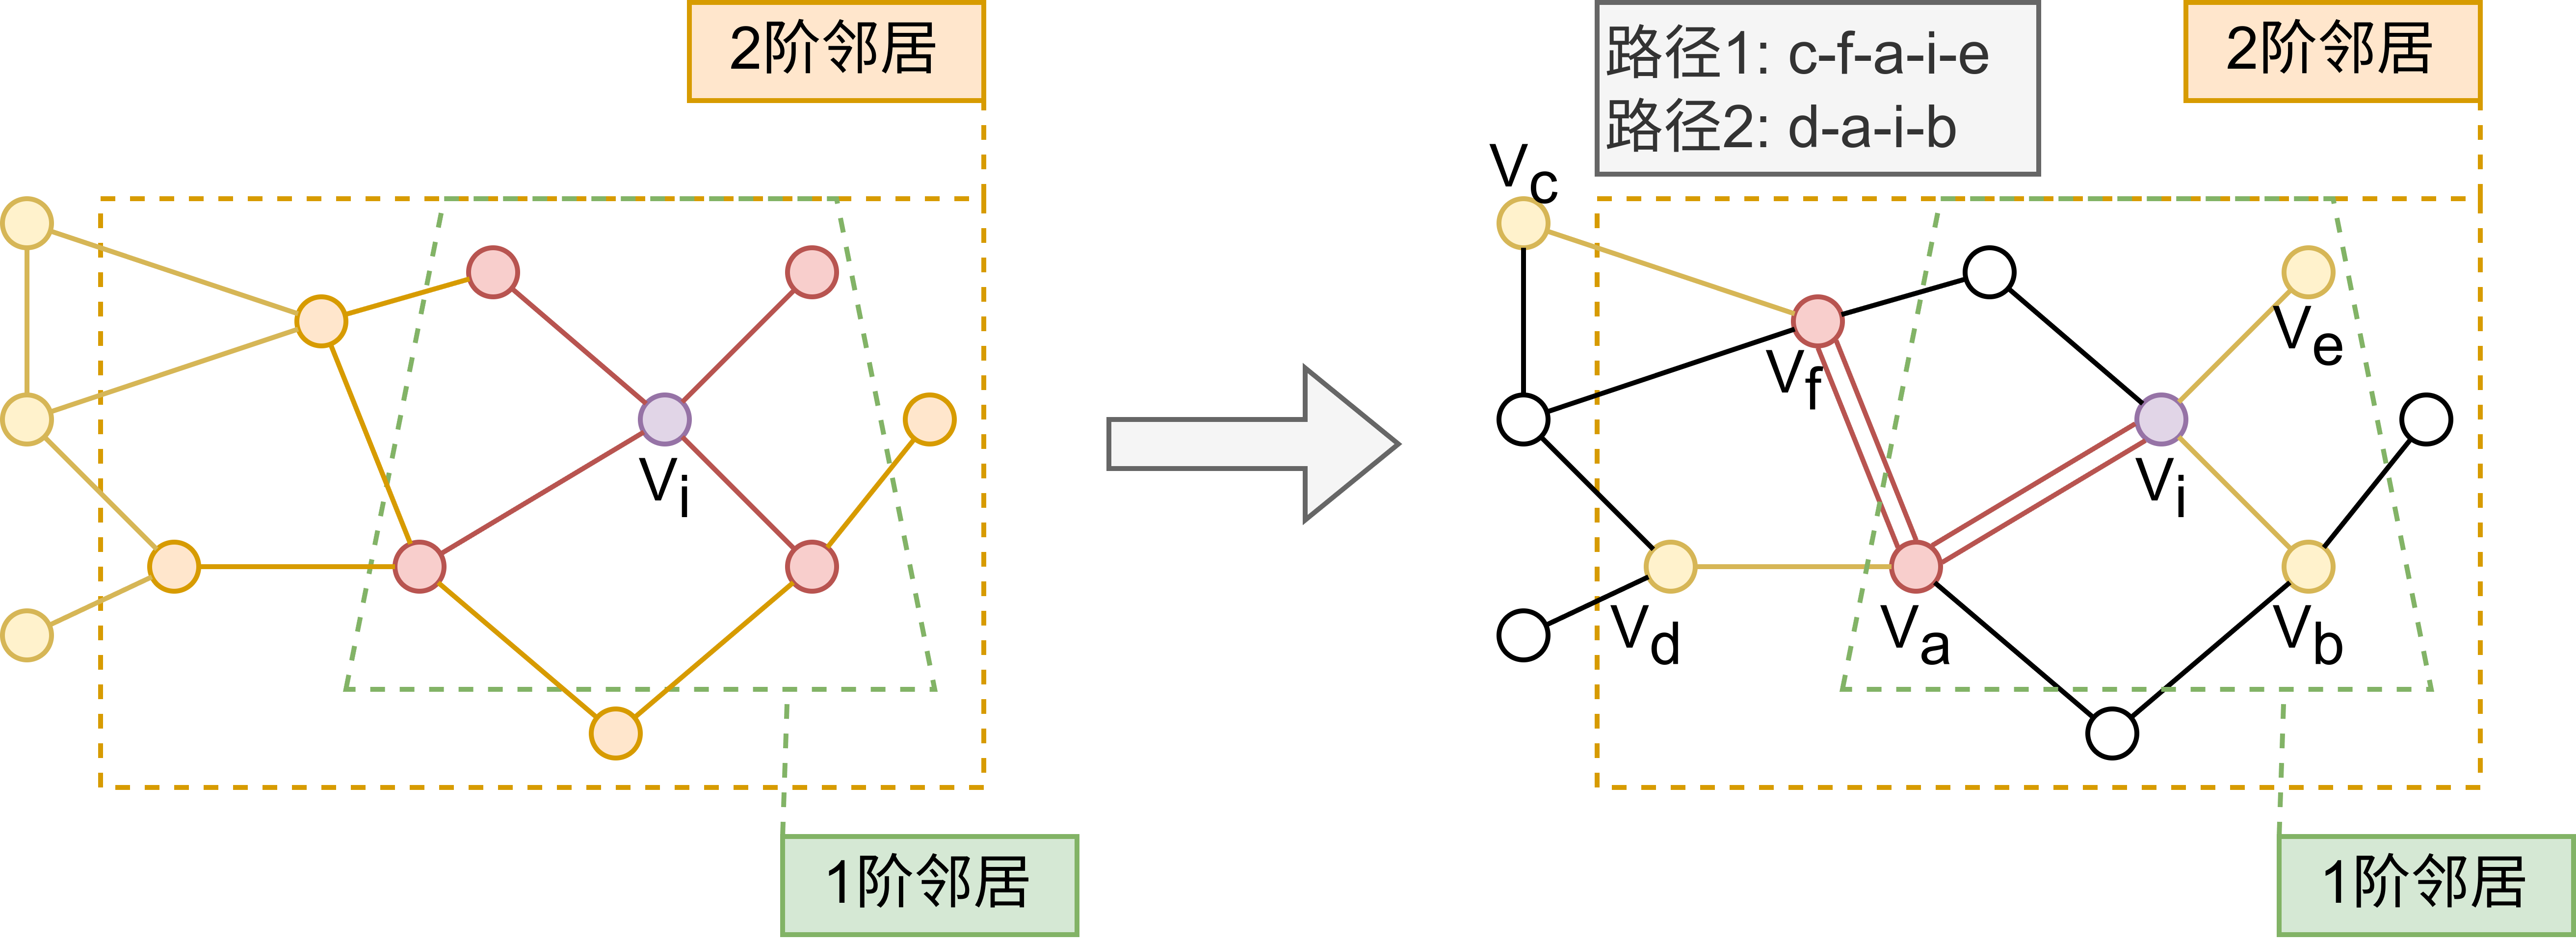
\includegraphics[width=0.9\linewidth]{chapter/c4_images/c4_nei-agg.png}
    \caption{邻居聚合方式的对比}
    \label{c4_nei-agg}
\end{figure}

\subsection{基于路由特征的损失设定}

基于与上一节相同的原理,本研究需要对基于图的无监督损失函数进行修正,它的原始定义如公式\ref{graphsage_default_loss}所示。
\begin{equation} \label{graphsage_default_loss}
J_G(Z_u) = -log(\sigma(z_u^{T}z_v)) - Q \cdot E_{v_n \sim P_n(v)}log(\sigma(-z_u^{T}z_v))
\end{equation}

它从当前节点的临接节点中采样对数损失,而从非临接节点中采样负的对数损失。该函数在 GraphSAGE 模型中被提出\citing{hamilton2017inductive},并被解释为一种实现在嵌入结果中相似嵌入节点更加接近的方法。

在本研究所述模型中,通过上述方式进行无监督的损失计算同样将抹去邻居间由路径产生的的差异,因而需要进行调整以适应存在路径特征的情形。

利用与上一节构造基于路径的聚合函数的方法可以设计一种损失函数,使得它能够可控地使得在同一条路径上的节点嵌入存在相似性,它的实现方式具体如公式\ref{graphsage_model_loss1}与公式\ref{graphsage_model_loss2}所示。
\begin{equation} \label{graphsage_model_loss1}
J(Z_u) = J_G(Z_u) + \theta_{loss} J_P(Z_u)
\end{equation}
\begin{equation} \label{graphsage_model_loss2}
J_P(Z_u) = -Q \cdot E_{v_n \sim P_{inpath}(v)}log(\sigma(z_u^{T}z_v)) -Q \cdot E_{v_n \sim P_{\sim inpath}(v)}log(\sigma(-z_u^{T}z_v))
\end{equation}

其中 $E_{v_n \sim P_{inpath}(v)}$ 表示在同一路径上的节点,即通过路径关联的节点;而 $E_{v_n \sim P_{\sim inpath}(v)}$ 表示不在同一路径上的节点,即互不通过路径关联的节点。

该损失公式通过结合图网络拓扑上的邻居损失 $J_G(Z_u)$ 和路径拓扑上的邻居损失 $J_P(Z_u)$,使得不仅相邻节点的嵌入更加相似,并且更多位于同一路径的节点(即路径意义上的邻居)应当在拓扑上更加相似。其中,$\theta_{loss}$ 控制了两种策略的比重,通过调整 $\theta_{loss}$ 的值能够使得节点更趋向与遵循基于路径的嵌入或是遵循基于网络拓扑的嵌入,而在具体损失的计算上依然沿用一般无监督学习所使用的对数损失函数,这在将模型运用于一些较少层次性的分布式网络中时能够适应其特点。

\subsection{异常检测方法}

在获得对应的节点嵌入后,对于需要检测的路由更新 $R_a$ 中路径的各节点 $V_i \in P_a \in R_a$ 获得对应的嵌入 ${e_i}$,并计算沿其路径相邻节点间的差异之和,此处使用如式\ref{negsim}所示的负对数相似度公式计算异常分数。
\begin{equation} \label{negsim}
D_a = \Sigma(||e_i - e_{i-1}||)
\end{equation}
在获得该值后即可通过设定一定的阈值以检测异常,即通过公式\ref{threshold}所描述的方法筛选大于 $\theta_{threshold}$ 的异常分数:
\begin{equation} \label{threshold}
p_{anomaly} = \{ \Sigma(||e_i - e_{i-1}||), v_i \in P_{input} \} \geq \theta_{threshold}
\end{equation}

然而,由于广域网络中的路由异常可能由正常操作导致,例如计划中的拓扑结构的改变,一般设置较低的阈值并对异常数值采取 top-k 的方式获得异常路由列表以供后续人工分析。

\section{实验及分析}

本章节的实验环节使用与前一章节相同的有标记数据集。首先,本研究设置了一组对照实验,通过准确度和时间度量对比在不同数据集下不同图网络模型的结果值,用于探究模型在横向和纵向两个维度下对异常检测性能的提升效果;由于模型包含数个参数值,本章节还设置了多组步进参数的参数分析实验,以探究模型在参数选取上对异常检测结果的影响;最后,为了证实模型引入的几个关键方法的有效性,本文设置了一组消融实验,将其各部分与对应的基线函数进行了比较。

\subsection{数据集设置}

为了验证使用了基于路径的采样方法的具体表现,本章实验使用未经预处理的大型互联网路由数据集,具体地,本章实验使用 RIPE RIS 在 2017 和 2022 的两个路由异常事故中带有具体异常时间标记的真实路由数据集作为模型的输入,同时使用了 2022 年有异常标记的 DN42 路由数据集作为小批量数据的输入对照,一些基本参数已在先前的表 \ref{c3_data_input} 中列出。

\subsection{对比实验}

\subsubsection{实验设置}

作为对照,本章节将使用 GraphSAGE 模型和传统的 GCN 模型,在上述数据集中进行比较,将异常标记时间段1天前的数据作为参考输入进行模型的训练,然后将异常标记时间内的流式路由更新数据作为对照的异常检测的输入数据。此实验使用异常检测精确度和 F-1 作为模型评价指标,以异常分数 0.5 为异常阈值进行判断。除此之外,为了反映性能上的提升,还将统计实验完整运行(包括图网络构建/生成、图的嵌入、异常检测等步骤)的平均耗时作为运行效率提升的衡量指标。

在图的采样上,采用 $\theta_{sample} = \theta_{loss} = 1$ 的方式进行采样,即对图结构与路径两类因素赋予相同的权重,并设置采样规模 $N_{sample} = 6$。

\subsubsection{实验结果}
% 耗时

在完整运行上述模型后,将异常检测结果汇总统计,表格 \ref{c4_s3tab1} 展示了不同模型在x种数据集下的性能表现和对应的效率表现,由此可以得到以下发现:

\begin{enumerate}
    \item 本章模型在各数据集上的异常检测效果均优于原始模型,与 GCN 模型接近,对比常规 GraphSAGE 模型而言有接近 10\% 的提升,这说明了模型在引入路径特征之后具有更好的异常检测性能。
    \item 本章模型和常规 GraphSAGE 模型的运行效率相近,相比 GCN 模型而言,依然能够保证有较大的运行效率提升,证明了模型的采样方法是高效的。
    \item 模型在 DN42 分布式网络数据集中的表现不如在 RIPE RIS 互联网数据集,一种可能的解释是在分布式网络数据自身在不同节点上的属性相似度较高,因而路由路径数据对邻居相似度的影响相比更弱。
\end{enumerate}

\begin{table}
    \caption{对比实验结果}
    \begin{tabular}{lccccccccc}
        \toprule
                  & \multicolumn{3}{l}{RIPE.2017} & \multicolumn{3}{l}{RIPE.2022} & \multicolumn{3}{l}{DN42.2022}                                               \\ \cmidrule(lr){2-4} \cmidrule(lr){5-7} \cmidrule(lr){8-10}
        模型        & Acc.                          & F-1                           & 运行时间                          & Acc.  & F-1   & 运行时间 & Acc.  & F-1   & 运行时间 \\ \midrule
        GCN       & 0.821                         & 0.817                         & 732s                          & 0.832 & 0.829 & 769s & 0.791 & 0.780 & 25s  \\
        GraphSAGE & 0.779                         & 0.763                         & 112s                          & 0.785 & 0.771 & 114s & 0.742 & 0.725 & 12s  \\
        本章模型      & 0.846                         & 0.837                         & 162s                          & 0.836 & 0.820 & 165s & 0.803 & 0.794 & 19s  \\
        \bottomrule
    \end{tabular}
    \label{c4_s3tab1}
\end{table}

\subsection{参数分析}

模型在上述对比实验中设置了对应的采样规模 $N_{sample}$、采样参数 $\theta_{sample}$ 和损失计算参数 $\theta_{loss}$,为了研究不同参数对结果的影响,以及研究最佳的参数值的决定方式,本文还对该模型进行了参数分析实验。

\subsubsection{实验设置}

在本实验中,在模型的训练阶段,上述三个参数将被分别以一定的步进独立地进行调整,在调整具体某个参数时,其它参数将被固定在对比实验的默认值,训练好的模型将被输入已被标记为异常的时间段内的路由更新,以进行路由异常的检测。本次实验采用 RIPE RIS 在 2022 年带标记的路由异常事故中的数据集,模型同样采用异常发生1天前的数据作为正常训练样本。

\subsubsection{实验结果}

通过以上方式进行实验,将数据汇总至如图 \ref{c4_arg-result} 所示的折线图内,从图中能够针对模型的参数得出几个结论:

\begin{enumerate}
    \item 在一定范围内,提升采样规模 $N_{sample}$ 有助于提升模型性能,这实质上是通过增大采样子图的尺寸来实现的,在极端状况($N_{sample}$足够大)下的模型与一般消息传递的图神经网络无异,因而此参数的提升将增加图网络的计算量且存在饱和的可能。
    \item 在采样参数 $\theta_{sample}$ 和损失参数 $\theta_{loss}$ 上,可见存在与数据集对应的最优值,这是由于数据集自身在节点嵌入属性上具有的与路径和图网络的相关性决定的。
    \item $\theta$ 参数在一定范围内的增加均有助于提升模型的表现,这反映了本章模型引入数据集中基于路径特征的权重的必要性。
\end{enumerate}

\begin{figure}[h]
    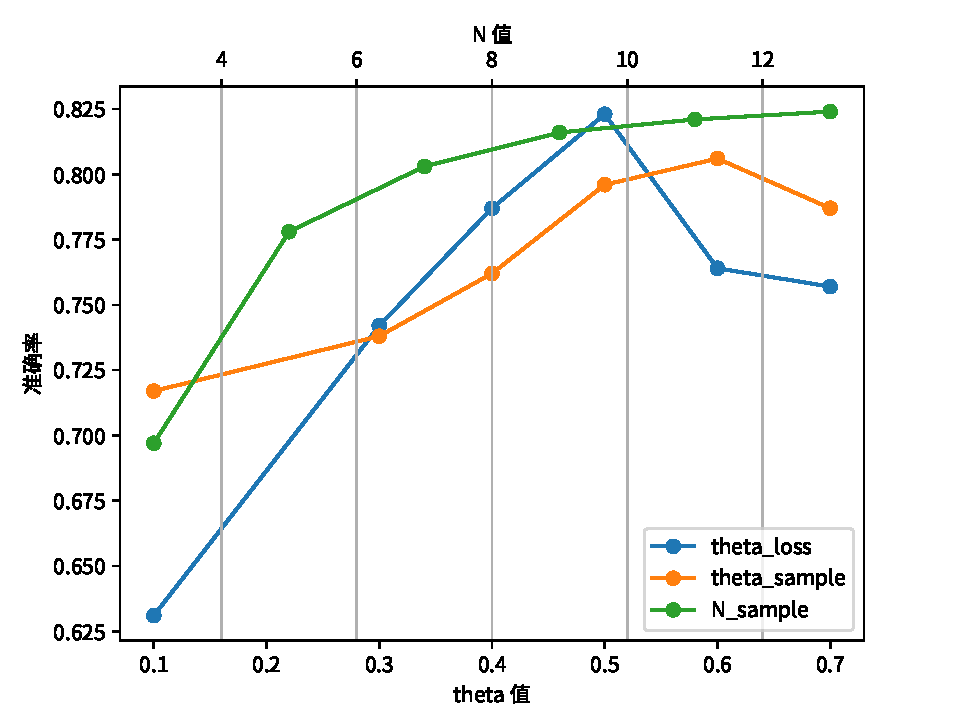
\includegraphics[width=0.9\linewidth]{chapter/c4_images/c4_arg-result.pdf}
    \caption{参数分析实验结果}
    \label{c4_arg-result}
\end{figure}

\subsection{消融实验}

本研究在 GraphSAGE 模型的基础上引入了独特的几种采样、聚合和计算损失的方式,为了验证其有效性,本研究为该模型设置了一组消融实验,该实验将展示这几类引入的算法在何种程度上提升了模型的最终效果。

\subsubsection{实验设置}

在消融实验中,作为对本章所述模型的消融对比,将在 GraphSAGE 模型的基础上替换采样函数、聚合函数和损失函数为各类基线函数,并采用与本章对比实验一致的参数设置,使用同样的数据集进行训练和测试。

实验一共针对模型中的三部分各自设置了三组对照:

\begin{enumerate}
    \item 对于邻居采样方法,设置了完全随机采样和以路径数量采样两种对照方法,对应研究在未引入路径因素和仅考虑路径因素的采样方法的条件下模型的性能变化。
    \item 针对聚合函数,设置了两组在 GraphSAGE 中常用的聚合方法\citing{hamilton2017inductive}作为对照,分别是均值聚合函数和归纳式均值聚合函数。
    \item 对于损失函数,消融实验设置了基于邻居嵌入最小化距离和路径嵌入最小化距离两种对照函数,分别对应于本模型中损失函数的两个极端情况。
\end{enumerate}

\subsubsection{实验结果}

消融实验的结果如表格 \ref{c4_s3tab2} 所示,它反映出了如下的一些特点:

\begin{enumerate}
    \item 本研究引入的基于路径的采样函数、聚合函数和损失函数均在提升异常检测性能上有一定贡献,总的来说,同时引入以上三种方式的模型的提升相比更大,这说明了本章在 GraphSAGE 三个方向提出的方法均在提升异常检测效果上具有作用。
    \item 在损失函数中引入基于路径的因素对模型的影响相比而言更大,一种可能的解释是,损失函数决定了训练参数的目标值,而采样和聚合方法自身在原理具有一定的随机性,从而在模型检测效果上的提升相对较少。
    \item 合理的设置参数 ($\theta$) 能够更好的提升模型异常检测的性能,这是由于在恰当的参数设置下,模型同时引入了路径和图的拓扑上的特征,过大或过小地设定参数将导致单一因素占据决定性比重,从而失去部分特征提取能力。
\end{enumerate}

\begin{table}
    \caption{消融实验结果}
    \begin{tabular}{lcccccc}
        \toprule
                        & \multicolumn{2}{l}{RIPE.2017} & \multicolumn{2}{l}{RIPE.2022} & \multicolumn{2}{l}{DN42.2022}                                                    \\ \cmidrule(lr){2-3} \cmidrule(lr){4-5} \cmidrule(lr){6-7}
        模型              & Acc.                          & F-1                           & Acc.                          & F-1            & Acc.           & F-1            \\ \midrule
        本章所述模型          & \textbf{0.846}                & \textbf{0.837}                & \textbf{0.836}                & \textbf{0.820} & \textbf{0.803} & \textbf{0.794} \\
        \midrule
        邻居采样                                                                                                                                                               \\
        \quad 完全随机采样    & 0.762                         & 0.759                         & 0.774                         & 0.771          & 0.750          & 0.752          \\
        \quad 以路径数量采样   & 0.795                         & 0.783                         & 0.799                         & 0.791          & 0.773          & 0.762          \\
        \midrule
        聚合函数                                                                                                                                                               \\
        \quad 均值聚合函数    & 0.749                         & 0.747                         & 0.752                         & 0.748          & 0.733          & 0.731          \\
        \quad 归纳式均值聚合函数 & 0.745                         & 0.743                         & 0.746                         & 0.744          & 0.730          & 0.735
        \\
        \midrule
        损失函数                                                                                                                                                               \\
        \quad 基于邻居嵌入最小化 & 0.721                         & 0.732                         & 0.725                         & 0.731          & 0.734          & 0.720          \\
        \quad 基于路径嵌入最小化 & 0.793                         & 0.790                         & 0.785                         & 0. 783         & 0.784          & 0.776
        \\
        \bottomrule
    \end{tabular}
    \label{c4_s3tab2}
\end{table}

\section{本章小结}
本章从路由数据的规模出发,研究基于采样和邻居聚合的图网络嵌入方案,并在 GraphSAGE 模型的基础上提出了一套利用数据集的路径属性进行节点嵌入的方法。在 4.1 节,介绍了现有基于图神经网络在大规模图数据上的不足和 GraphSAGE 模型框架在运用于路径式数据上的不足。在 4.2 节,通过对模型进行分析,本文针对 GraphSAGE 模型的三个基本模块进行了探讨,设计出了利用路径特征的对应方法。在 4.3 节,为了验证以上方法在改善原有模型效果上的有效性,进行了对照实验,然后通过消融实验评估了模型在不同设计下的性能。